\documentclass[11pt]{article}
\usepackage[T1]{fontenc}
\usepackage{lmodern}
\usepackage{amsmath,amssymb,amsthm,mathtools}
\usepackage{graphicx}
\usepackage[margin=1in]{geometry}
\usepackage[colorlinks=true,linkcolor=blue,citecolor=blue,urlcolor=blue]{hyperref}
\usepackage{microtype}

\newtheorem{theorem}{Theorem}
\newtheorem{lemma}[theorem]{Lemma}
\newtheorem{remark}[theorem]{Remark}
\newcommand{\K}{\mathbb K}
\newcommand{\N}{\mathbb N}
\newcommand{\card}{\operatorname{Card}}

\title{Two ultrametric answers:\\
sharp Grothendieck constant and failure of restricted invertibility\\
\large Full answers to Problems 1.4 and 3.2 in arXiv:2503.20972}
\author{Automated mathematics discovery run \texttt{fa\_banach\_001}\\
Lane 5, candidate for human review}
\date{19 July 2026}

\begin{document}
\maketitle

\begin{center}
\fbox{\parbox{0.92\textwidth}{\textbf{Status: candidate full solution, likely valid.}
Problem 1.4 holds over every non-Archimedean valued field with the sharp
constant $K_{\K}=1$.  Problem 3.2 is false over every such field.  This
packet does not claim an answer to Problem 1.5 or Problem 2.5.}}
\end{center}

\section{The source problems}

Krishna asks three families of questions motivated by classical Euclidean
inequalities \cite{Kri}.  The first target here is Problem 1.4: under a
normalized scalar bilinear estimate, does the corresponding inner-product
estimate hold uniformly over all $p$-adic Hilbert spaces?  The complete
source statement is reproduced below.

\begin{center}
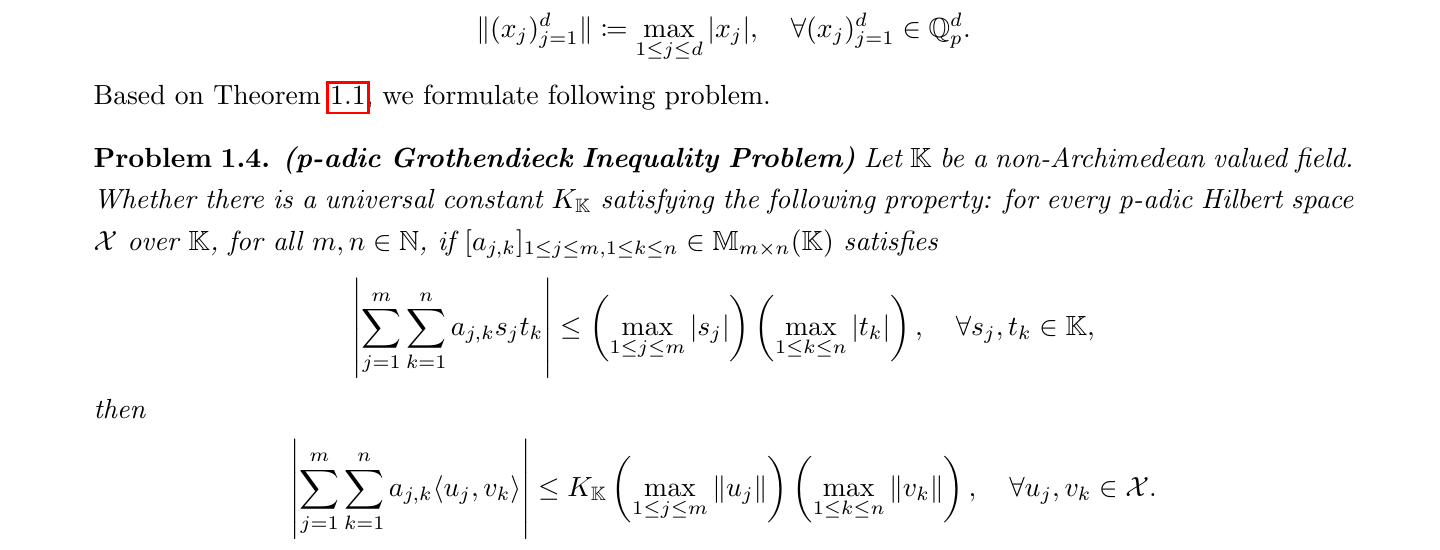
\includegraphics[width=0.98\textwidth]{figures/grothendieck_problem_crop.png}
\end{center}

The second target is Problem 3.2, the proposed non-Archimedean analogue of
the Bourgain--Tzafriri restricted-invertibility theorem.

\begin{center}
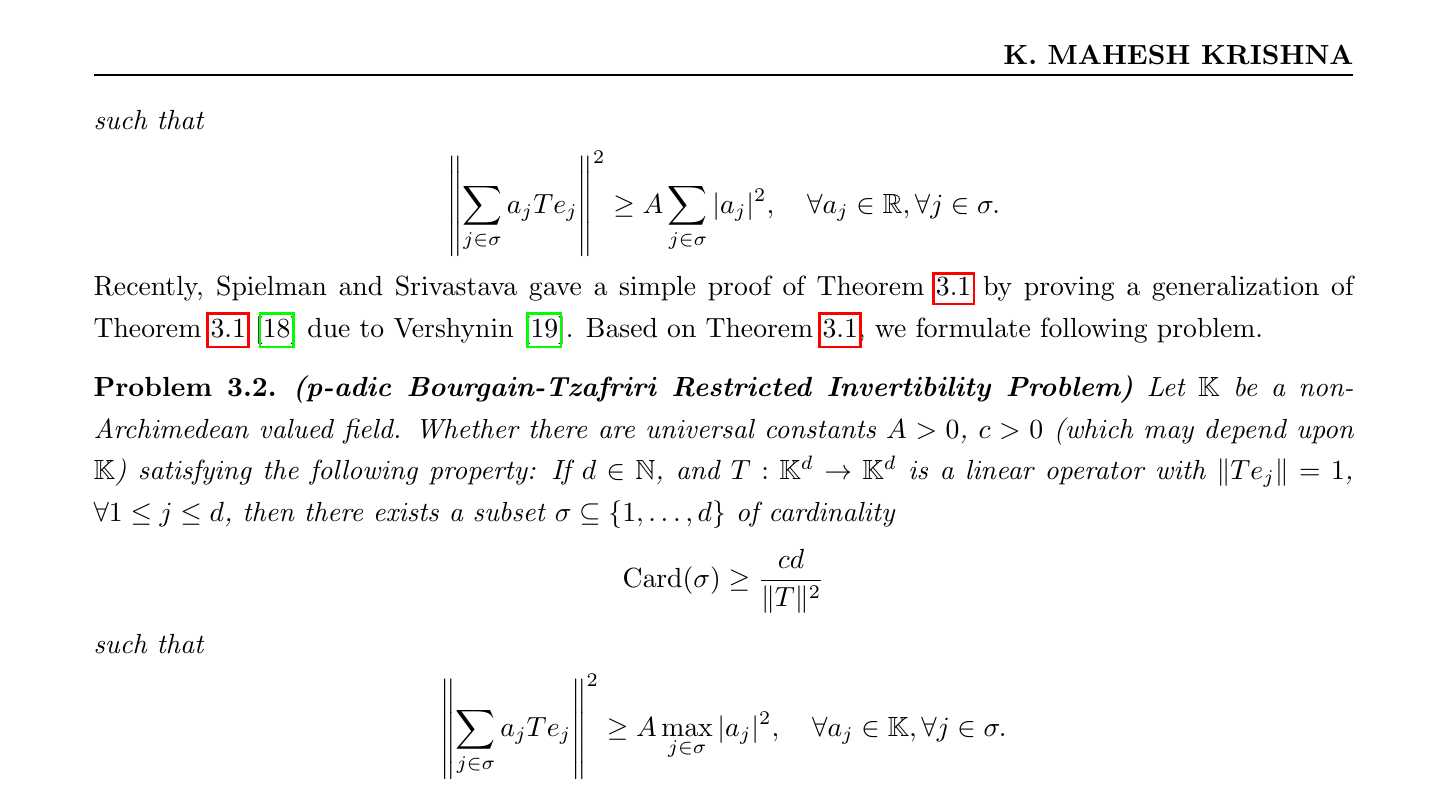
\includegraphics[width=0.98\textwidth]{figures/restricted_invertibility_problem_crop.png}
\end{center}

Throughout, $\K^d$ carries the standard maximum norm
$\lVert x\rVert_\infty=\max_j|x_j|$, as in the source's finite-dimensional
model.

\section{Results}

\begin{theorem}[Sharp normalized Grothendieck inequality]\label{thm:groth}
Let $\K$ be any non-Archimedean valued field and let $\mathcal X$ be any
$p$-adic Hilbert space over $\K$ in the sense of \cite{Kri}.  Suppose
$A=(a_{j,k})\in\mathbb M_{m\times n}(\K)$ satisfies
\begin{equation}\label{eq:scalar-hyp}
 \left|\sum_{j=1}^m\sum_{k=1}^n a_{j,k}s_jt_k\right|
 \le \left(\max_j|s_j|\right)\left(\max_k|t_k|\right)
 \qquad(s_j,t_k\in\K).
\end{equation}
Then, for all $u_j,v_k\in\mathcal X$,
\begin{equation}\label{eq:vector-conclusion}
 \left|\sum_{j=1}^m\sum_{k=1}^n
 a_{j,k}\langle u_j,v_k\rangle\right|
 \le \left(\max_j\lVert u_j\rVert\right)
      \left(\max_k\lVert v_k\rVert\right).
\end{equation}
Consequently Problem 1.4 has the optimal answer $K_{\K}=1$ for every $\K$.
\end{theorem}

\begin{theorem}[Failure of p-adic restricted invertibility]\label{thm:bt}
Let $\K$ be any non-Archimedean valued field.  There do not exist positive
real constants $A,c$ satisfying the assertion in Problem 3.2, even when the
constants are allowed to depend on $\K$.
\end{theorem}

\section{Proof intuition}

Both answers have the same cause.  In a non-Archimedean norm, a sum is no
larger than its largest summand.  Thus a normalized scalar Grothendieck
hypothesis bounds every matrix entry separately, and no dimension-dependent
accumulation remains in the vector-valued sum.  The best constant collapses
to one.

The same maximum principle makes restricted invertibility fail dramatically.
Arbitrarily many identical unit columns define an operator of norm one: their
sum still cannot exceed the largest input coordinate.  But every restriction
containing two columns has a nontrivial kernel.  Hence the proposed stable-rank
cardinality lower bound and injective lower estimate cannot coexist.

\section{Proof of Theorem~\ref{thm:groth}}

Let $e_j\in\K^m$ and $e_k\in\K^n$ denote coordinate vectors.  Substitute
$s=e_j$ and $t=e_k$ in \eqref{eq:scalar-hyp}.  Since zero coordinates are
permitted, this gives
\begin{equation}\label{eq:entry-bound}
             |a_{j,k}|\le 1 \qquad(1\le j\le m,\ 1\le k\le n).
\end{equation}
The strong triangle inequality, \eqref{eq:entry-bound}, and axiom (iv) in the
source's definition of a $p$-adic Hilbert space now give
\begin{align*}
 \left|\sum_{j,k}a_{j,k}\langle u_j,v_k\rangle\right|
 &\le \max_{j,k}|a_{j,k}|\,|\langle u_j,v_k\rangle|\\
 &\le \max_{j,k}\lVert u_j\rVert\,\lVert v_k\rVert\\
 &=\left(\max_j\lVert u_j\rVert\right)
   \left(\max_k\lVert v_k\rVert\right).
\end{align*}
This proves \eqref{eq:vector-conclusion} with $K_{\K}=1$.

The constant cannot be smaller.  Take the one-dimensional $p$-adic Hilbert
space $\mathcal X=\K$, put $m=n=1$, and take
$a_{1,1}=u_1=v_1=1$.  The scalar hypothesis holds and both sides of
\eqref{eq:vector-conclusion} equal one.  This proves sharpness.

\begin{remark}\label{rem:equiv}
The argument also shows that the scalar hypothesis \eqref{eq:scalar-hyp} is
equivalent to the entrywise condition $\max_{j,k}|a_{j,k}|\le1$.  The reverse
implication follows immediately from the strong triangle inequality.  This
is precisely where the normalized non-Archimedean problem differs from its
Archimedean analogue.
\end{remark}

\section{Proof of Theorem~\ref{thm:bt}}

For each $d\in\N$, define $T_d:\K^d\to\K^d$ by
\begin{equation}\label{eq:T}
 T_d(x_1,\ldots,x_d)=\left(\sum_{j=1}^d x_j\right)e_1.
\end{equation}
Every column is the same unit vector:
\begin{equation}\label{eq:columns}
                    T_de_j=e_1,\qquad \lVert T_de_j\rVert_\infty=1.
\end{equation}
Moreover, ultrametricity gives
\[
 \lVert T_dx\rVert_\infty
 =\left|\sum_{j=1}^d x_j\right|
 \le\max_j|x_j|=\lVert x\rVert_\infty.
\]
Thus $\lVert T_d\rVert\le1$, while equality holds at $x=e_1$; hence
\begin{equation}\label{eq:opnorm}
                         \lVert T_d\rVert=1.
\end{equation}

Suppose for contradiction that Problem 3.2 held with some fixed $A,c>0$.
Choose an integer $d$ such that $cd\ge2$ and apply it to $T_d$.  By
\eqref{eq:opnorm}, the promised set $\sigma$ would satisfy
\[
             \card(\sigma)\ge \frac{cd}{\lVert T_d\rVert^2}=cd\ge2.
\]
Choose distinct $j,k\in\sigma$, set $a_j=1$, $a_k=-1$, and set all other
$a_i$ to zero.  From \eqref{eq:columns},
\[
       \sum_{i\in\sigma}a_iT_de_i=e_1-e_1=0,
       \qquad \max_{i\in\sigma}|a_i|^2=1.
\]
The demanded estimate would therefore read $0\ge A$, contradicting $A>0$.
This proves Theorem~\ref{thm:bt}.

The cancellation is valid in every characteristic.  In characteristic two,
$-1=1$, but $1+(-1)=0$ and $|-1|=1$ still hold.

\section{Scope and novelty check}

Theorem~\ref{thm:groth} answers Problem 1.4 only.  Problem 1.5 constrains
every scalar test coordinate to have modulus one, so the coordinate probes
with zeros used in \eqref{eq:entry-bound} are unavailable; no answer to that
formulation is claimed here.

Problem 2.5 prints the same factor $1-\varepsilon$ in its lower and upper
distortion bounds, apparently a typographical error.  We neither correct nor
exploit that display.  Theorem~\ref{thm:bt} answers Problem 3.2 exactly as
printed.

The run's cheap indexes were searched by arXiv identifier, exact title, and
the core problem phrases.  A bounded primary arXiv search found the source
paper but no later resolution of either problem.  This is not an exhaustive
novelty certification.

\begin{thebibliography}{9}
\bibitem{Kri}
K. Mahesh Krishna,
\emph{p-adic Grothendieck Inequality, p-adic Johnson--Lindenstrauss
Flattening and p-adic Bourgain--Tzafriri Restricted Invertibility Problems},
arXiv:2503.20972v3 (2026).
\end{thebibliography}

\end{document}
